\section{Descripción de los experimentos}
Usaremos la función f(x)=cos(x) para desarrollar nuestro experimento.

\begin{figure}[!th]
\begin{center}
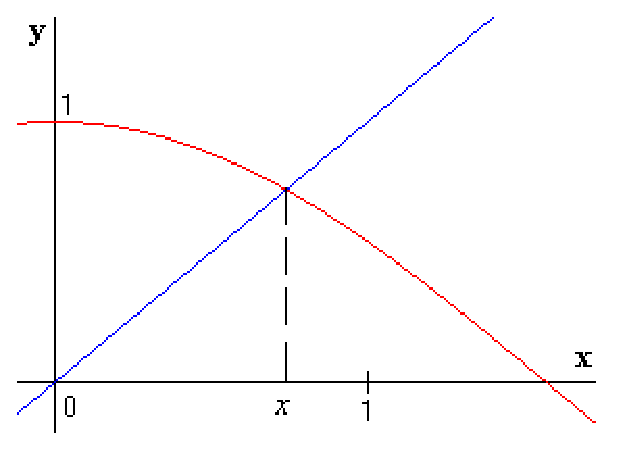
\includegraphics[width=0.25\textwidth]{images/metodo25.eps}
\caption{Gráfico 1}
\end{center}
\end{figure}

En el primer gráfico podemos observar las representaciones de las dos funciones que utilizaremos
asi como la coordenada de la abscisa de su punto de intersección en el primer cuadrante. Para hallar 
la abscisa del punto de intersección basta con igualar las funciones de la siguiente manera:
x=cos(x), entonces igualamos a cero la ecuación: $cos(x)-x = 0.$


\begin{figure}[!th]
\begin{center}
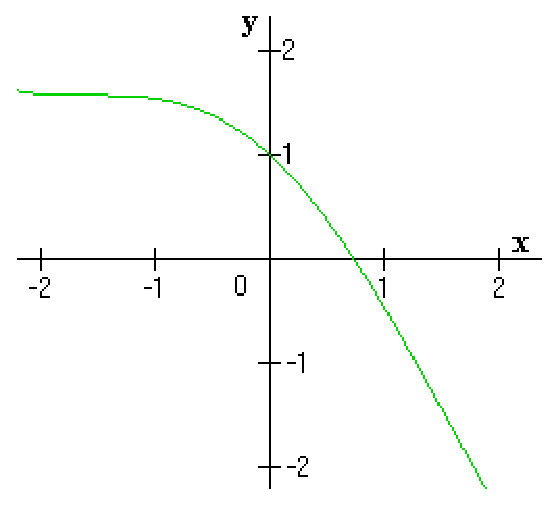
\includegraphics[width=0.25\textwidth]{images/metodo26.eps}
\caption{Gráfico 2}
\end{center}
\end{figure}

En el grafico 2 vemos la representación de la funcion $f(x)=cos(x)-x$
Ahora utilizaremos el Método de Newton para hallar, con una aproximación de 4 cifras decimales, el cero: \\

\centerline{$ x_{n+1} = x_n - \frac{f(x_n)}{f'(x_n)}, f'(x_n)!= 0  \hspace{2cm}(*)$}   
\vspace{0.5cm}

Sea:\\

\centerline{$f(x)=cos(x)-x \hspace{0.5cm}(1) \hspace{0.5cm}\rightarrow f'(x)=-sen(x)-1 \hspace{2cm}(2)$}
\vspace{0.5 cm}

De (*), (1) y (2) se deduce que la segunda aproximacion esta dada por:\\

\centerline{$ x2 = x1- \frac {(cos(x)-x)}{(-sen(x)-1)} = x1 + \frac {(cos(x)-x)}{(sen(x)+1)} \hspace{2cm}(3)$}
\vspace{0.5 cm} 


Fijandonos en la grafica de f, escogemos a x1=1. 
Ahora:\\

\centerline {$f(1)=-0, 4597 \hspace{2cm} (2)$} 
\centerline {$f'(1)= 1,8415 \hspace{2cm} (6)$}
\vspace{0.5 cm}

Sustituyendo (4),(5) y (6) en (3), se obtiene:\\

\centerline {$ x2 = 1 + \frac {(-0,4597)}{1,8415} \rightarrow x2 = 0,7504 $}
\vspace{0.5 cm}

Para este nuevo valor de x, calculamos:\\

\centerline {$f(0,7504) = -0,0109 $}
\centerline {$ f'(0,7504) = 1,6819 $}
\vspace{0.5 cm}

De tal manera que:\\

\centerline {$x3 = 0,7504 + \frac {(-0.0109)}{1.6819} = 0.7391 \hspace{2cm}(7)$}
\vspace{0.5 cm}

Para este nuevo valor de x, calculamos:\\

\centerline {$f(0.7391) = 0 $}
\centerline {$f'(0.7391) = 1.6736 $}
\vspace{0.5 cm}

De tal manera que:\\

\centerline {$x4 = 0.7391 - \frac {0} {1.6736} = 0.7391   \hspace{2cm}(8)$}
\vspace{0.5 cm}

Comparando (7) y (8), se tiene que:\\

\centerline {$x3=x4=0.7391$}
\vspace{0.5 cm}

La coordenada x del punto de intersección en el primer cuadrante de las graficas es x=0.7391 

Por ultimo, en este primer apartado de descripción experimental es necesario poner un codigo python que satisfaga nuestro experimento y constituye el siguiente:

\begin{verbatim}
while(x != tempo and i<100):
     tempo = x
     x = x- funcionDada(x)/derivadaFuncionDada(x)
     e = abs ((x-tempo)/x)

     print("x" + str(i) + "=" + str(x) + "error=" + str(e) + "\n")
     i=i+1
\end{verbatim}



\section{Descripción del material}
En este apartado, hablaremos sobre el material en el cual hemos realizado nuestro experimento.

Nuestro experimento ha sido realizado en un PC con la versión del sistema operativo(S.O.):\\

\leftline{'Linux-3.2.0-61-generic-i686-with-Ubuntu-12.04-precise'}
%('default', 'Feb 27 2014 20:00:17')
\vspace{0.5cm}


El tipo de compilador que hemos utilizado para nuestro experimento es el del lenguaje de programacion Python :\\ 

\centerline{'2.7.3'}
%('Linux', 'galois00', '3.2.0-61-generic', '#93-Ubuntu SMP Fri May 2 21:33:33 UTC 2014', 'i686', 'i686')
\vspace{0.5cm}

Y, por último, los datos que aparecen a continuacion, hacen referencia al hardware de la maquina:\\
\begin{itemize}
\item Pentium(R) Dual-Core  CPU      E5200  @ 2.50GHz
\item GenuineIntel
\item 1200.000 Hz 
\item 2048 KB
\end{itemize}

Todos los lectores de este informe, se preguntaran de cómo hemos obtenido estos datos, pues se le ha de informar que estos datos han sido obtenidos gracias a un código Python(que guarda los datos en un fichero) que es el siguiente:

\begin{verbatim}
def SOFTinfo():
  softinfo=()
  softinfo={'Several':platform.uname(),'S.O':platform.platform(),
 'Pythons Version':platform.python_version(), 'Date':platform.python_build()}
  return softinfo
\end{verbatim}



\section{Resultados obtenidos}
En este apartado de {\bf Resultados obtenidos} debemos darle un valor al codigo Python mostrado en páginas anteriores y observar los distintos valores del error. A continuacion mostraremos una tabla con los valores del punto $x_0$ y los errores obtenidos, dándole el valor 1 a la x.
\begin{table}[!ht]
\begin{center}
\begin{tabular}{|c|l|l|}
\hline
     $x_0$     &      error        \\ \hline
0.496558178297 & 7.04158813835     \\ \hline
2.13100384448  & 1.2330160875      \\ \hline
0.689662720778 & 2.089972175491    \\ \hline
0.739652997531 & 0.0675861206807   \\ \hline
0.739085204376 & 0.000768237751393 \\ \hline
0.739085133215 & 9.62821076424e-08 \\ \hline
0.739085133215 & 1.50215851291e-15 \\ \hline
0.739085133215 & 0.0               \\ \hline

\end{tabular}
\end{center}
\caption{Tabla de errores}
\end{table}

Seguidamente vamos a exponer la grafica de los errores, realizada mediante el programa matplolib. Esta figura tiene dos graficas, una ampliada con los errores al completo, y otra mas reducida, sin los tres primeros x y errores.
\begin{figure}[!th]
\begin{center}
\includegraphics[width=0.6\textwidth]{images/Grafica_de_errores.eps}
\caption{Gráfico de errores}
\end{center}
\end{figure}

Para realizar esta grafica, hemos empleado un coigo python, que es el siguiente:
\begin{verbatim}

hola.plot(x,y,"r*")
hola.title('Grafica de errores ampliada')
hola.ylabel('error')
hola.ylim(-0.4,7.3)
hola.xlim(0.48,2.2)

\end{verbatim}


\section{Analisis de resultados}
Al realizar el programa en Python para resolver el metodo de Newton aplicado a la funcion $f(x)=cos(x)$ y obtener los resultados de la tabla anteriormente expuesta, pudimos apreciar que se obtienen una serie de errores según se le iban dando valores a la "x", pudimos ver una cierta curiosidad, la cual dandole casi el mismo valor a la x; 
0.739652997531, 0.739085204376 y 0.739085133215(este se da 3 veces, pero es porque el programa redondea en ese numero), se producen errores muy diferentes ya que unos son de $\frac {1}{10^8}$ y otros de $0.000768237751393$.\\
Tambien se puede observar que cuanto mayor sea el valor de la "x", mayor es el error, excepto en el caso de $x_0 =0.496558178297$ cuyo error es 7.0415881385 y $x_1=2.13100384448$ cuyo error es 1.2330160875.\\
Tambien observamos que al insertar x mayores, es decir, $x=6$, $x=7$, $x=8$, etc, se producen muchos más valores de $x_n$ y por lo tanto, muchos mas errores.\\ 
A partir de la grafica podemos ver la gran cercania de algunos puntos, que incluso ni se aprecian. \\
Segun los datos que hemos obtenido, podemos llegar a la conclusion de que, este metodo hace que la funcion tienda a cero, esto es, que los valores de los errores se aproximen cada vez mas a {\bf cero}. 
Este hecho, constrasta lo dicho en el apartado de fundamentos teoricos donde se expuso que f(x)=0 debido a la aplicación del metodo de Newton.
 